%!TEX root = ../main.tex

\chapter{HARQ}
\label{chp:harq}

\section{HARQ overview}
The main objective of telecommunication technologies is the transfer of information between different actors. Modern systems aim at an efficient usage of the available resources, while trying to meet all the necessary requirements of the application that is generating the data to be transferred. 

The \ac{HARQ} protocol hereby described helps achieve a more efficient use of the available resources when errors occur, using an intelligent system of retransmissions that, in turn, lowers the error rate at the expense of a higher latency.

The main building blocks of \ac{HARQ} are \ac{ARQ} and \ac{FEC}. The role of \ac{ARQ} is to automatically request the retransmission of the whole packet when the receiver detects the presence of errors, while \ac{FEC} is tasked to correct such errors using redundancy bits added to the packet by the transmitter. The joint operation of those two protocols makes the foundation of \ac{HARQ}, currently in use in all the most popular network standards such as 4G, Wi-Fi and 5G \cite{3gpp-38-series}. \ac{HARQ} peculiarity resides in the fact that it avoids the retransmission of the whole packet in case of errors, preferring to send additional redundant information to help the decoding process.

\section{Concurrent processes limit}
\label{sec:harq-conc-proc}

One of the problems highlighted by the \ac{3GPP} technical report \cite{3gpp-tr-38.811} on the matter of non-terrestrial networks regards the maximum number of concurrent \ac{HARQ} processes. 

\subsection{Problem description}
The details of \ac{HARQ} protocol implementation in the 5G \ac{NR} standard is extensively treated in many publications such as \cite{harq-wireless-communications-survey}. However, for the purpose of understanding what is a \ac{HARQ} process and how it affects the throughput in a non-terrestrial scenario, a brief overview of a few key concepts is enough.

\begin{figure}[ht]
    \centering
    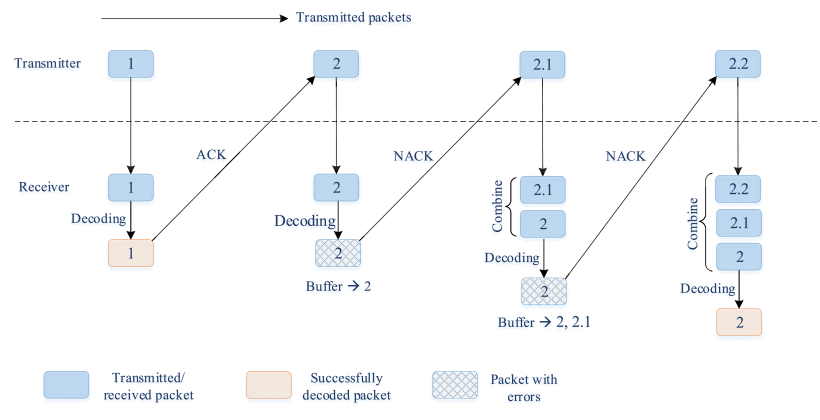
\includegraphics[width=0.9\textwidth]{res/harq-retx-scheme.png}
    \caption{\ac{HARQ} retransmission diagram \cite{harq-wireless-communications-survey}}
    \label{fig:harq_retx_scheme}
\end{figure}

\subsubsection{HARQ working principle}
\paragraph{}
Fig. \ref{fig:harq_retx_scheme} gives an overview of how \ac{HARQ} processes work. Upon successful reception, depicted in the first column of Fig. \ref{fig:harq_retx_scheme}, an \ac{ACK} is sent back, triggering the transmission of the successive \ac{TB}, which is represented in the second column. This behavior is the normal state in which transmissions are received correctly, and it keeps repeating itself until errors are detected.

\paragraph{} Should the receiver detect errors in the received \ac{TB}, represented by the greyed packet, a \ac{NACK} is relayed back to the sender, which in turn proceeds to send some additional redundancy bits. Note that the sender does not repeat the whole \ac{TB}. The receiver now proceeds to decode the transfer block using all the information that it has received so far.

This is the most important feature of \ac{HARQ} protocol: it does not discard the packets affected by errors, since they can be at least used to recover some information. The erroneous packets are stored in buffers and used for joint decoding \cite{5g-nr-harq-devopedia}. 

\paragraph{} If the redundancy bits that the sender just transmitted are still not enough to allow for a correct decoding of the transfer block, or if another error is detected, a retransmission is triggered. This is shown in the last column of Fig. \ref{fig:harq_retx_scheme}, where all the packets received so far contribute in correctly decoding packet 2.

Finally, if even this retransmission is affected by errors and the combination of the information received so far is not enough to complete the decoding of the \ac{TB}, additional information is sent. After this fourth interaction, no further attempts are made to correct the packet \cite{5g-nr-harq-sharetechnote}.

\paragraph{} The various transmissions and retransmissions being made by the protocol are called \ac{RV}, and are numbered from 0 to 3. Their order can vary depending on the implementation and configuration. Figure \ref{fig:harq_retx_scheme_2} shows another example where the redundancy versions are ordered as 0, 3, 2.

\begin{figure}[ht]
    \centering
    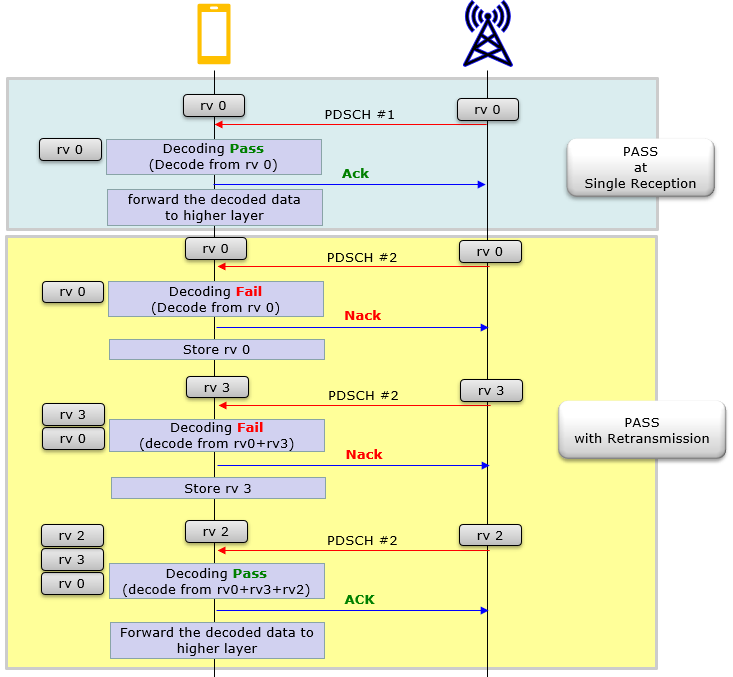
\includegraphics[width=0.9\textwidth]{res/harq-retx-scheme-2.png}
    \caption{\ac{HARQ} diagram with different RVs\cite{5g-nr-harq-sharetechnote}}
    \label{fig:harq_retx_scheme_2}
\end{figure}


\subsubsection{Stop and wait}
\paragraph{} The presented behavior means that \ac{HARQ} is a stop-and-wait kind of protocol, since it is designed to wait for the arrival of previous packet's \ac{ACK} before sending the new one. While this enforces the delivery of ordered packets, it also brings the downside of severely underutilizing the channel capacity, wasting resources that could potentially be used for transmission instead \cite{3gpp-ts-38.214}. Figures \ref{fig:harq_retx_scheme_2} and \ref{fig:harq_retx_scheme} highlight this pattern.

This limitation is overcome by the introduction of multiple concurrent processes.

\subsubsection{Processes}
\paragraph{}
A \ac{HARQ} process starts when a \ac{TB} is passed to the \ac{HARQ} entity and finishes when the \ac{ACK} relative to that same \ac{TB} is received by the sender. After the \ac{ACK} is correctly received, the next \ac{TB} starts being processed. Considering a link with propagation delay $\tau_p$, the minimum active time for a process is therefore $2\tau_p$, i.e. the time for the transfer block to arrive to the destination plus the time for the acknowledgement to travel back to the sender.

The 5G \ac{NR} standard allows the base station to configure the maximum number of concurrent \ac{HARQ} processes to be assigned to each connected user, with the default value being of 8 concurrent processes and the maximum 16 \cite{3gpp-ts-38.300, 5g-nr-harq-devopedia}. In this way it is possible to partially limit the effects of the stop-and-wait behavior, allowing for a better throughput.

\subsubsection{Application in NTNs}
\paragraph{}
Since the propagation delay of \ac{NTNs} is order of magnitude larger than their terrestrial counterpart, the limited maximum number of concurrent processes lowers the maximum achievable throughput, as detailed in the following toy example. 

\paragraph{Example} Consider a scenario where each process tries to send a \ac{TB} every $2\tau_p$, which is the maximum rate at which transfer blocks can be sent under the condition of waiting for the acknowledgement to arrive before starting a new transmission. The other endpoint is a \ac{LEO} satellite orbiting at 2.000Km, therefore having $\tau_p\approx6$ms. Assuming the best possible conditions with no need for retransmissions and assuming that the base station grants the \ac{UE} to the best possible clearance of 16 concurrent processes, the total send rate is of 16 transfer blocks every 12ms. In order to target a throughput of 50Mbps, the block size must therefore be of at least $$\frac{\textit{target throughput} \times 2\tau_p}{\textit{number of processes}} = 37,5Kb$$
Doing the same calculation for a terrestrial scenario with the \ac{gNB} placed at a distance of 600m from the \ac{UE}, we obtain that the minimum \ac{TBS} must be of just $12b$.
Both calculations do not factor in overheads, control information, channel access requests and processing delays, but are helpful to give an idea of the disproportion in place between the two conditions.

While the necessary block size for the \ac{NTN} case is technically possible to achieve even with the older 4G technology, it necessitates a high \ac{SNR} to work properly. This constraint becomes even more conservative in the non-terrestrial case, since retransmissions add delays in multiples of the propagation delay and can therefore quickly become a lot more costly \cite{4g-phy-processing-sharetechnote}.

\subsection{Possible solutions}
\label{sec:proc-harq-prop-sol}
\paragraph{Increasing the processes}
The easiest solution would be to increase the number of maximum concurrent \ac{HARQ} processes. However, this comes with some caveats mainly regarding the higher computational capabilities required and higher power consumption, that can quickly become problematic in battery-operated equipments such as smartphones. Each process also requires the presence of a buffer on both the receiver side and the sender side, so additional resources are required at the \ac{gNB}, too. 
\paragraph{Aggressive HARQ}
A more sophisticated approach could involve the design of an aggressive version of the \ac{HARQ} protocol, where each process is allowed to send multiple packets before receiving an acknowledgement. Since there already are multiple concurrent processes, each \ac{ACK} packet must already contain a field specifying the number of process it belongs to, and the information identifying the specific packet to be acknowledged within a process could be encoded inside this field.
\paragraph{Disable \ac{HARQ}}
Lastly, the option of disabling \ac{HARQ} completely and rely solely on \ac{ARQ} retransmissions has been proposed by 3GPP itself \cite{hybrid-arq-schemes-muk}. This, however, would come with a performance penalty since satellite links typically suffer from more severe conditions than terrestrial ones, and \cite{5g-beyond-5g-ntn-trends-vanellicoralli} demonstrated that a version of \ac{HARQ} specifically designed for non-terrestrial networks would be beneficial.

\subsection{Implemented solution - More processes}
\subsubsection{Testing current implementation}
\paragraph{}
To test the practical effect that the concurrent processes' limitation has on the achievable throughput, a simulation campaign was conducted where the \ac{HARQ} protocol was firstly disabled and successively enabled, therefore obtaining results for the two different scenarios. The maximum number of concurrent processes with \ac{HARQ} enabled was set to 16, that is the maximum that a \ac{gNB} can allocate to each \ac{UE}.

\paragraph{}
Comparing the obtained results confirmed that employing \ac{HARQ} caused a noticeable negative impact on the throughput, as can be appreciated in Fig. \ref{fig:harq_on_off}. The throughput without \ac{HARQ} perfectly matches the source rate, since the \ac{SNR} values of this simulation are high enough to correctly deliver almost the totality of the packets. 

On the other hand, the throughput with \ac{HARQ} enabled reaches its plateau as the source rate crosses the 4Mb/s threshold, settling at this value. \ac{HARQ} struggles to keep up with the increasing source rate since the limited number of processes starts to cause packets to be dropped whenever a retransmission is needed. For a high enough source rate, the \ac{HARQ} protocol is completely overwhelmed, as all the 16 processes are always busy, and the arriving packets that do not find an available process are promptly discarded.


\begin{figure}[ht]
    \centering
    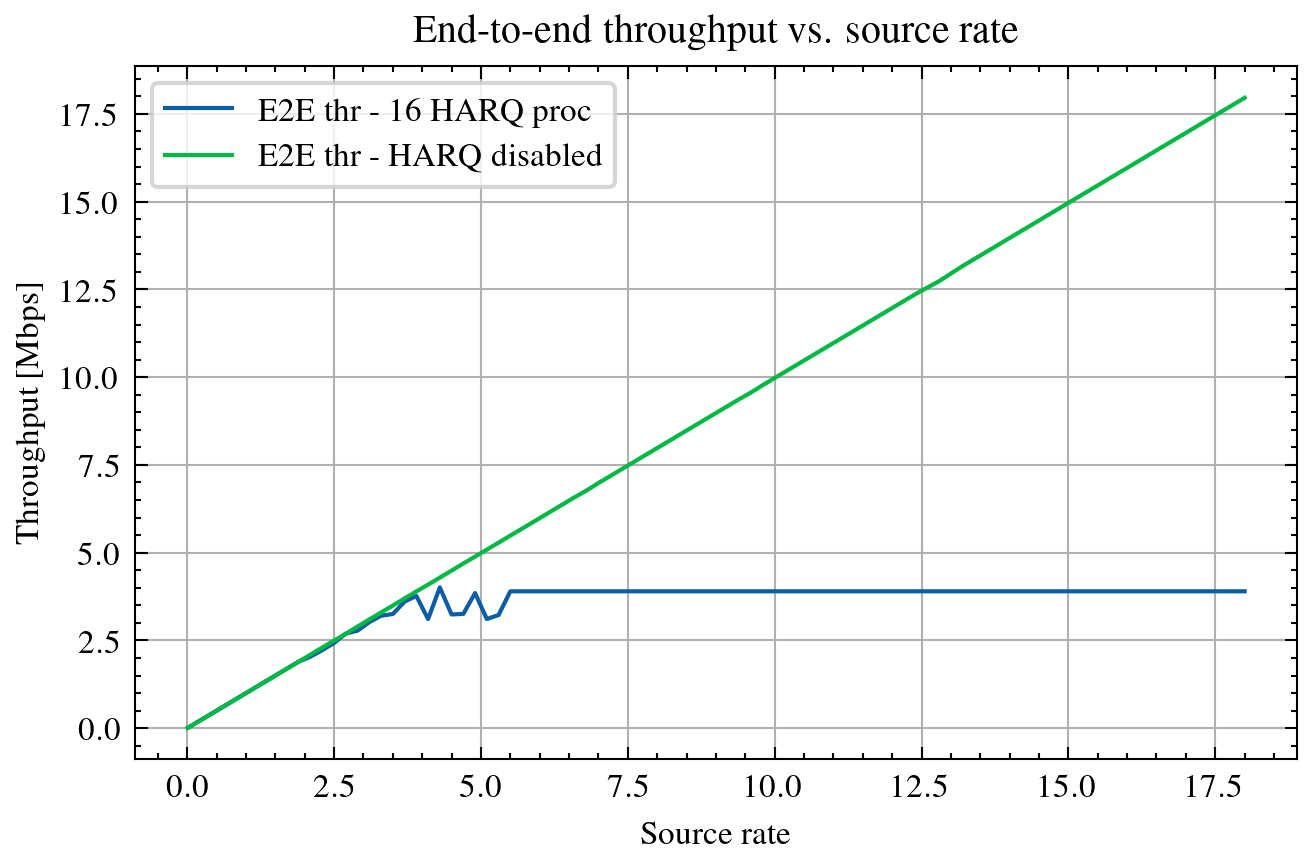
\includegraphics[width=0.9\textwidth]{res/harq-onoff2.png}
    \caption{End-to-end throughput comparison with and without \ac{HARQ}, $\tau_p=6$ms.}
    \label{fig:harq_on_off}
\end{figure}

\paragraph{}
Having verified that \ac{HARQ} does indeed limit the achievable throughput, a modification was implemented to the protocol suite to manually force a higher number of concurrent processes. The simulation campaign was then re-run and the results are shown in Fig. \ref{fig:harq-numproc}.

\begin{figure}[ht]
    \centering
    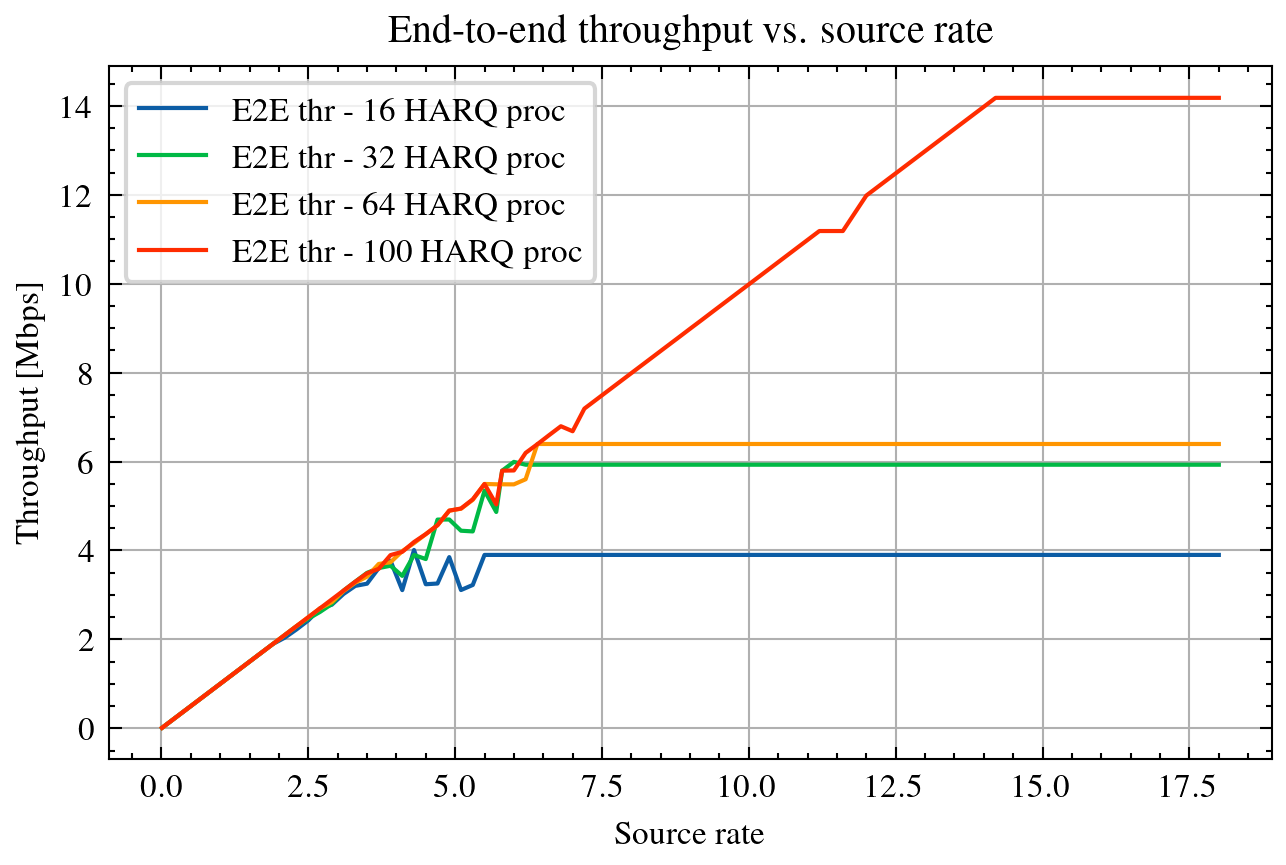
\includegraphics[width=0.9\textwidth]{res/harq_numproc_new.png}
    \caption{End-to-end throughput comparison with different number of concurrent \ac{HARQ} processes, $\tau_p=6$ms.}
    \label{fig:harq-numproc}
\end{figure}

\subsubsection{Results}
\paragraph{}
Increasing the allowed processes pushed the maximum achievable throughput to just over 14Mb/s in the scenario with the highest allowance of per-user concurrent processes. Going past such threshold causes packets to start being dropped, and the throughput to saturate, since there are no more available processes to send the traffic generated by the application.

The results shown in figure \ref{fig:harq-numproc} make clear that increasing the parameter regulating the number of \ac{HARQ} processes allows for higher speeds. Each line in the plot was obtained with a different number of allowed processes, starting from 16, the maximum allocable value in the 5G \ac{NR} standard, then 32, 64 and ultimately 100. No further increases have been evaluated, since those would currently be unrealistic to achieve.

However, constraints regarding the required computational power and the increased energy consumption shall also be taken into careful consideration, since raising the number of concurrent processes from 16 to 100 is a big step, bringing a consistent increase in both the receiver and transmitter complexity with it.

We can conclude that, while certainly being a way to improve the performances of \ac{HARQ} in non-terrestrial scenarios, the increase in processes alone cannot solve the problem of \ac{HARQ} limiting the throughput, therefore other ways have to be found, and future studies should also consider alternative proposals.

\subsection{Implemented solution - Disabling HARQ}
\paragraph{}
Figure \ref{fig:harq_on_off} could suggest that completely disable the \ac{HARQ} protocol could be a viable solution, since the end to end throughput of the simulation with \ac{HARQ} switched off always matched the source rate, meaning that all the packets generated by the application were correctly received by the remote host.

However, the reason of this behavior is the high \ac{SNR} that was forced in the simulated scenario with the choice of using high gain antennas. This design choice is not fully realistic, since the intended final use case of non-terrestrial networks is their usage with mobile handsets. Such choice was made because this work is focused on the study of the propagation delay, and the high gain of aperture antennas allowed to limit the impact of the problems caused by low \ac{SNR}. Having a communication channel with high \ac{SNR} allowed for fewer variables to impact the simulations' results, in turn enabling the study of propagation delay alone.

\paragraph{}
In order to test the performances without \ac{HARQ} enabled, a new simulation campaign has been conducted factoring in the problems related to poor \ac{SNR}, such as the presence of errors in the received packets and the need for retransmissions. In conditions of low \ac{SNR}, which can be plausible in a non-terrestrial communication scenario, the \ac{PDR} and therefore the throughput can drop considerably, impacting the link reliability.
\paragraph{}
Simulations have shown that fully disable \ac{HARQ} may be a good solution only when both \ac{UE} and \ac{gNB} experience optimal channel conditions with high \ac{SNR}, while poor channel conditions may benefit from having \ac{HARQ} enabled.

A hybrid approach can also be thought, where \ac{CQI} can be used to assess the state of the channel and decide whether to enable \ac{HARQ}, therefore limiting the throughput in exchange for a higher reliability, or disabling it, should the \ac{SNR} be high enough.

\iffalse
    \subsection{Simulator configuration}
    While the number of concurrent HARQ processes can be configured in ns-3, it cannot exceed the value of 100. By performing some simple calculations, knowing that the \ac{SNR} conditions allow for the transmissions of \ac{TB}s with size of 1024B, to achieve a target throughput of 50Mbps on the best case of 6ms $\tau_p$ the necessary processes would be 74.
    $$\frac{\textit{target throughput} \times 2\tau_p}{\textit{total block size}} \approx 74 \textit{processes}$$

    This does not account for the delays caused by retransmissions, so simulator crashes due to processes overflow are frequent while testing even the best case scenario.

\fi

